%\documentclass{beamer} 
\documentclass[handout]{beamer} % sin pausas
\usetheme{CambridgeUS}

\usepackage{etex}
\usepackage{t1enc}
\usepackage[spanish,es-nodecimaldot]{babel}
\usepackage{latexsym}
\usepackage[utf8]{inputenc}
\usepackage{verbatim}
\usepackage{multicol}
\usepackage{amsgen,amsmath,amstext,amsbsy,amsopn,amsfonts,amssymb}
\usepackage{amsthm}
\usepackage{calc}         % From LaTeX distribution
\usepackage{graphicx}     % From LaTeX distribution
\usepackage{ifthen}
%\usepackage{makeidx}
\input{random.tex}        % From CTAN/macros/generic
\usepackage{subfigure} 
\usepackage{tikz}
\usepackage[customcolors]{hf-tikz}
\usetikzlibrary{arrows}
\usetikzlibrary{matrix}
\tikzset{
    every picture/.append style={
        execute at begin picture={\deactivatequoting},
        execute at end picture={\activatequoting}
    }
}
\usetikzlibrary{decorations.pathreplacing,angles,quotes}
\usetikzlibrary{shapes.geometric}
\usepackage{mathtools}
\usepackage{stackrel}
%\usepackage{enumerate}
\usepackage{enumitem}
\usepackage{tkz-graph}
\usepackage{polynom}
\polyset{%
    style=B,
    delims={(}{)},
    div=:
}
\renewcommand\labelitemi{$\circ$}
\setlist[enumerate]{label={(\arabic*)}}
%\setbeamertemplate{background}[grid][step=8 ] % cuadriculado
\setbeamertemplate{itemize item}{$\circ$}
\setbeamertemplate{enumerate items}[default]
\definecolor{links}{HTML}{2A1B81}
\hypersetup{colorlinks,linkcolor=,urlcolor=links}


\newcommand{\Id}{\operatorname{Id}}
\newcommand{\img}{\operatorname{Im}}
\newcommand{\nuc}{\operatorname{Nu}}
\newcommand{\im}{\operatorname{Im}}
\renewcommand\nu{\operatorname{Nu}}
\newcommand{\la}{\langle}
\newcommand{\ra}{\rangle}
\renewcommand{\t}{{\operatorname{t}}}
\renewcommand{\sin}{{\,\operatorname{sen}}}
\newcommand{\Q}{\mathbb Q}
\newcommand{\R}{\mathbb R}
\newcommand{\C}{\mathbb C}
\newcommand{\K}{\mathbb K}
\newcommand{\F}{\mathbb F}
\newcommand{\Z}{\mathbb Z}
\newcommand{\N}{\mathbb N}
\newcommand\sgn{\operatorname{sgn}}
\renewcommand{\t}{{\operatorname{t}}}
\renewcommand{\figurename }{Figura}

%
% Ver http://joshua.smcvt.edu/latex2e/_005cnewenvironment-_0026-_005crenewenvironment.html
%

\renewenvironment{block}[1]% environment name
{% begin code
	\par\vskip .2cm%
	{\color{blue}#1}%
	\vskip .2cm
}%
{%
	\vskip .2cm}% end code


\renewenvironment{alertblock}[1]% environment name
{% begin code
	\par\vskip .2cm%
	{\color{red!80!black}#1}%
	\vskip .2cm
}%
{%
	\vskip .2cm}% end code


\renewenvironment{exampleblock}[1]% environment name
{% begin code
	\par\vskip .2cm%
	{\color{blue}#1}%
	\vskip .2cm
}%
{%
	\vskip .2cm}% end code




\newenvironment{exercise}[1]% environment name
{% begin code
	\par\vspace{\baselineskip}\noindent
	\textbf{Ejercicio (#1)}\begin{itshape}%
		\par\vspace{\baselineskip}\noindent\ignorespaces
	}%
	{% end code
	\end{itshape}\ignorespacesafterend
}


\newenvironment{definicion}[1][]% environment name
{% begin code
	\par\vskip .2cm%
	{\color{blue}Definición #1}%
	\vskip .2cm
}%
{%
	\vskip .2cm}% end code

    \newenvironment{notacion}[1][]% environment name
    {% begin code
        \par\vskip .2cm%
        {\color{blue}Notación #1}%
        \vskip .2cm
    }%
    {%
        \vskip .2cm}% end code

\newenvironment{observacion}[1][]% environment name
{% begin code
	\par\vskip .2cm%
	{\color{blue}Observación #1}%
	\vskip .2cm
}%
{%
	\vskip .2cm}% end code

\newenvironment{ejemplo}[1][]% environment name
{% begin code
	\par\vskip .2cm%
	{\color{blue}Ejemplo #1}%
	\vskip .2cm
}%
{%
	\vskip .2cm}% end code


\newenvironment{preguntas}[1][]% environment name
{% begin code
    \par\vskip .2cm%
    {\color{blue}Preguntas #1}%
    \vskip .2cm
}%
{%
    \vskip .2cm}% end code

\newenvironment{ejercicio}[1][]% environment name
{% begin code
	\par\vskip .2cm%
	{\color{blue}Ejercicio #1}%
	\vskip .2cm
}%
{%
	\vskip .2cm}% end code


\renewenvironment{proof}% environment name
{% begin code
	\par\vskip .2cm%
	{\color{blue}Demostración}%
	\vskip .2cm
}%
{%
	\vskip .2cm}% end code



\newenvironment{demostracion}% environment name
{% begin code
	\par\vskip .2cm%
	{\color{blue}Demostración}%
	\vskip .2cm
}%
{%
	\vskip .2cm}% end code

\newenvironment{idea}% environment name
{% begin code
	\par\vskip .2cm%
	{\color{blue}Idea de la demostración}%
	\vskip .2cm
}%
{%
	\vskip .2cm}% end code

\newenvironment{solucion}% environment name
{% begin code
	\par\vskip .2cm%
	{\color{blue}Solución}%
	\vskip .2cm
}%
{%
	\vskip .2cm}% end code



\newenvironment{lema}[1][]% environment name
{% begin code
	\par\vskip .2cm%
	{\color{blue}Lema #1}\begin{itshape}%
		\par\vskip .2cm
	}%
	{% end code
	\end{itshape}\vskip .2cm\ignorespacesafterend
}

\newenvironment{proposicion}[1][]% environment name
{% begin code
	\par\vskip .2cm%
	{\color{blue}Proposición #1}\begin{itshape}%
		\par\vskip .2cm
	}%
	{% end code
	\end{itshape}\vskip .2cm\ignorespacesafterend
}

\newenvironment{teorema}[1][]% environment name
{% begin code
	\par\vskip .2cm%
	{\color{blue}Teorema #1}\begin{itshape}%
		\par\vskip .2cm
	}%
	{% end code
	\end{itshape}\vskip .2cm\ignorespacesafterend
}


\newenvironment{corolario}[1][]% environment name
{% begin code
	\par\vskip .2cm%
	{\color{blue}Corolario #1}\begin{itshape}%
		\par\vskip .2cm
	}%
	{% end code
	\end{itshape}\vskip .2cm\ignorespacesafterend
}

\newenvironment{propiedad}% environment name
{% begin code
	\par\vskip .2cm%
	{\color{blue}Propiedad}\begin{itshape}%
		\par\vskip .2cm
	}%
	{% end code
	\end{itshape}\vskip .2cm\ignorespacesafterend
}

\newenvironment{conclusion}% environment name
{% begin code
	\par\vskip .2cm%
	{\color{blue}Conclusión}\begin{itshape}%
		\par\vskip .2cm
	}%
	{% end code
	\end{itshape}\vskip .2cm\ignorespacesafterend
}


\newenvironment{definicion*}% environment name
{% begin code
	\par\vskip .2cm%
	{\color{blue}Definición}%
	\vskip .2cm
}%
{%
	\vskip .2cm}% end code

\newenvironment{observacion*}% environment name
{% begin code
	\par\vskip .2cm%
	{\color{blue}Observación}%
	\vskip .2cm
}%
{%
	\vskip .2cm}% end code


\newenvironment{obs*}% environment name
	{% begin code
		\par\vskip .2cm%
		{\color{blue}Observación}%
		\vskip .2cm
	}%
	{%
		\vskip .2cm}% end code

\newenvironment{ejemplo*}% environment name
{% begin code
	\par\vskip .2cm%
	{\color{blue}Ejemplo}%
	\vskip .2cm
}%
{%
	\vskip .2cm}% end code

\newenvironment{ejercicio*}% environment name
{% begin code
	\par\vskip .2cm%
	{\color{blue}Ejercicio}%
	\vskip .2cm
}%
{%
	\vskip .2cm}% end code

\newenvironment{propiedad*}% environment name
{% begin code
	\par\vskip .2cm%
	{\color{blue}Propiedad}\begin{itshape}%
		\par\vskip .2cm
	}%
	{% end code
	\end{itshape}\vskip .2cm\ignorespacesafterend
}

\newenvironment{conclusion*}% environment name
{% begin code
	\par\vskip .2cm%
	{\color{blue}Conclusión}\begin{itshape}%
		\par\vskip .2cm
	}%
	{% end code
	\end{itshape}\vskip .2cm\ignorespacesafterend
}






\newcommand{\nc}{\newcommand}

%%%%%%%%%%%%%%%%%%%%%%%%%LETRAS

\nc{\FF}{{\mathbb F}} \nc{\NN}{{\mathbb N}} \nc{\QQ}{{\mathbb Q}}
\nc{\PP}{{\mathbb P}} \nc{\DD}{{\mathbb D}} \nc{\Sn}{{\mathbb S}}
\nc{\uno}{\mathbb{1}} \nc{\BB}{{\mathbb B}} \nc{\An}{{\mathbb A}}

\nc{\ba}{\mathbf{a}} \nc{\bb}{\mathbf{b}} \nc{\bt}{\mathbf{t}}
\nc{\bB}{\mathbf{B}}

\nc{\cP}{\mathcal{P}} \nc{\cU}{\mathcal{U}} \nc{\cX}{\mathcal{X}}
\nc{\cE}{\mathcal{E}} \nc{\cS}{\mathcal{S}} \nc{\cA}{\mathcal{A}}
\nc{\cC}{\mathcal{C}} \nc{\cO}{\mathcal{O}} \nc{\cQ}{\mathcal{Q}}
\nc{\cB}{\mathcal{B}} \nc{\cJ}{\mathcal{J}} \nc{\cI}{\mathcal{I}}
\nc{\cM}{\mathcal{M}} \nc{\cK}{\mathcal{K}}

\nc{\fD}{\mathfrak{D}} \nc{\fI}{\mathfrak{I}} \nc{\fJ}{\mathfrak{J}}
\nc{\fS}{\mathfrak{S}} \nc{\gA}{\mathfrak{A}}
%%%%%%%%%%%%%%%%%%%%%%%%%LETRAS


\title[Clase 21 - Caminatas eulerianas]{Matemática Discreta I \\ Clase 21 - Caminatas eulerianas, ciclos hamiltonianos}
%\author[C. Olmos / A. Tiraboschi]{Carlos Olmos / Alejandro Tiraboschi}
\institute[]{\normalsize FAMAF / UNC
    \\[\baselineskip] ${}^{}$
    \\[\baselineskip]
}
\date[03/06/2021]{3 de junio de 2021}




\begin{document}
    
    \frame{\titlepage} 
    
    \begin{frame}\frametitle{Los puentes de Könisberg}
        
        {\color{blue}Pregunta}%
    \vskip .2cm
            ¿Es posible cruzar todos los puentes pasando  una y solo una vez por cada uno?         Leonhard Euler (1707-1783).
    
        
        \begin{figure}
            \includegraphics[scale=0.12]{images/konisberg_hc.png}
        \end{figure}
        
    \end{frame}
    
    
    \begin{frame}\frametitle{Los puentes de Könisberg - versión 2}
        \begin{figure}
            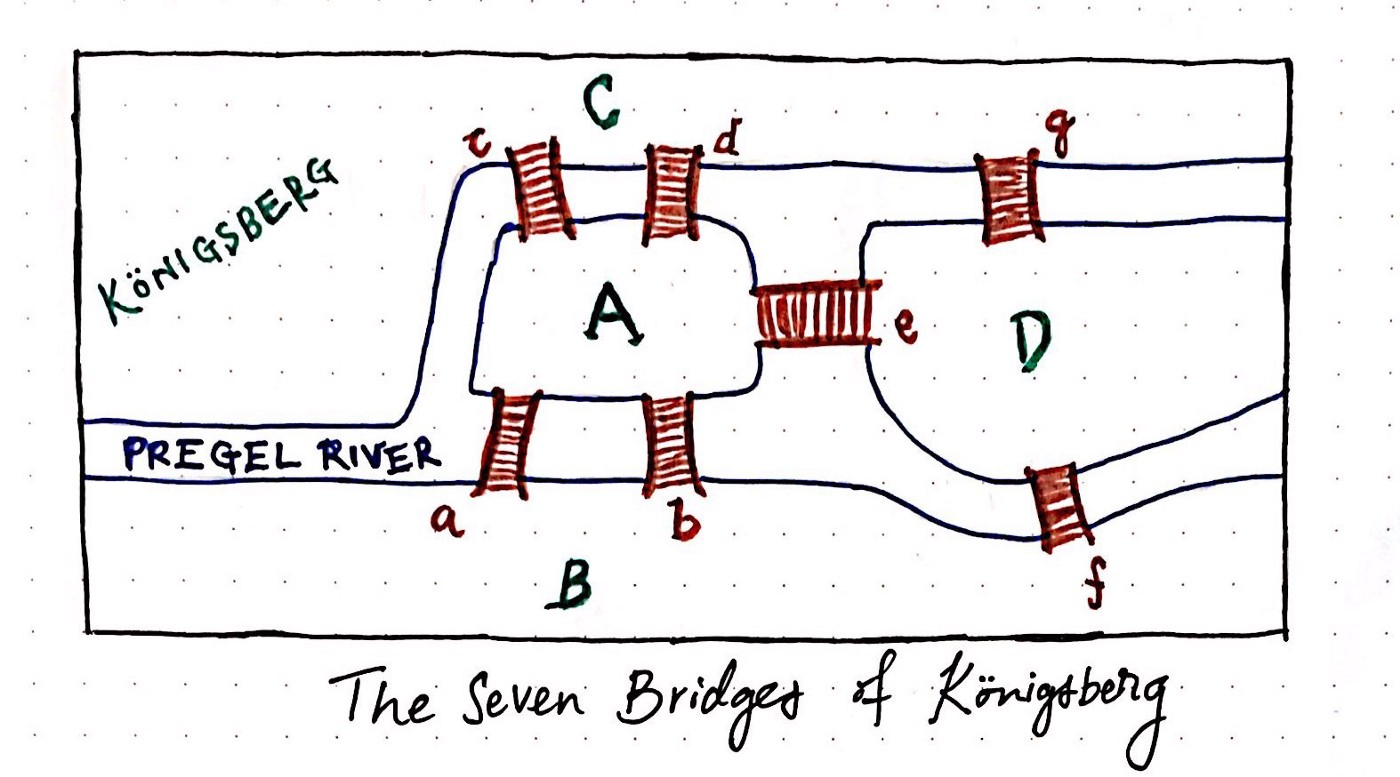
\includegraphics[scale=0.23]{images/konisberg2.jpg}
        \end{figure}
    \end{frame}
    
    \begin{frame}\frametitle{Los puentes de Könisberg - versión 3}
        \begin{figure}
            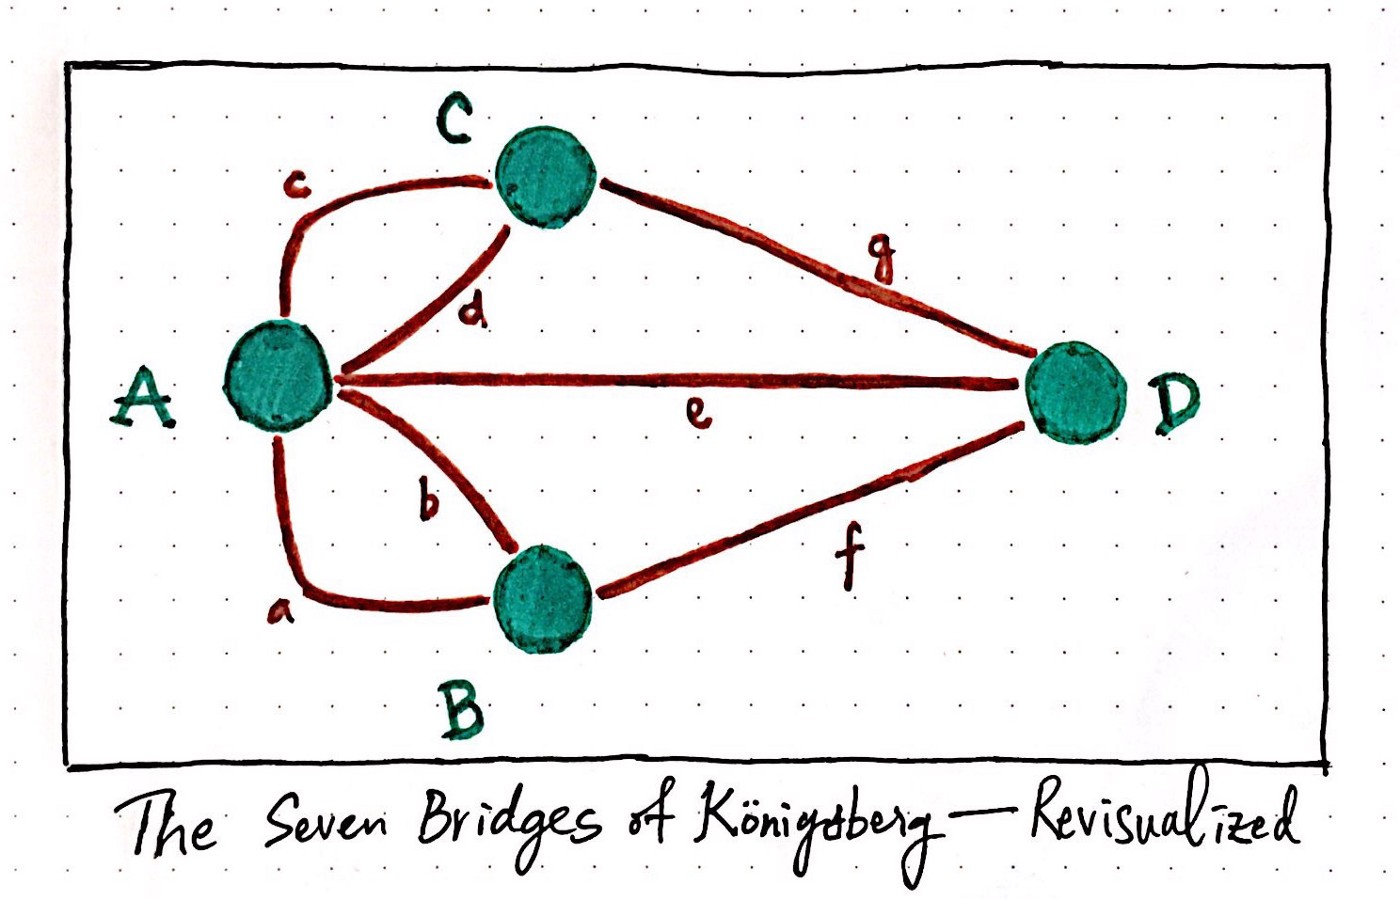
\includegraphics[scale=0.18]{images/konisberg3.jpg}
        \end{figure}
        
        Ahora el problema se reduce a encontrar una caminata  que use cada arista (o puente) una y solo una vez.
    \end{frame}
    
    \begin{frame}
        \begin{observacion}
            $\delta(A)=5$, $\delta(B)=3$, $\delta(C)=3$, $\delta(D)=3$.
        \end{observacion}
        
        \vskip .5cm
        
        Euler, abstrayéndose del problema concreto, razonó de la siguiente manera:
        
        \vskip .5cm 
        \begin{itemize}
            \item Supongamos que el vértice de partida es $x$ y  el de llegada es $y$. Todos los demás los llamo intermedios.
            \item En un vértice intermedio cada vez que entro por un puente salgo por otro. Eso  me ``aporta''  2 a la valencia.
            \item Terminado el proceso usé todos los puentes, por lo tanto  en cada vértice intermedio la cantidad de entradas más la cantidad de salidas es la valencia. Como la cantidad de entradas es igual a la cantidad de salidas, la valencia es par.
            
        \end{itemize}
        
        
    \end{frame}
    
    \begin{frame}
        \textbf{Concluyendo}
        \vskip .3cm
        \begin{itemize}
            \item Si hay una caminata que pasa por cada puente una y solo una vez,  la cantidad de vértices con valencia impar es a lo sumo 2. 
            \item Como todos los vértices en el problema tienen valencia impar, el problema no tiene solución. 
        \end{itemize}
        \vskip .3cm
        Como veremos más adelante el problema de los puentes de Könisberg puede ser generalizado y también vale la recíproca.
        \vskip .5cm
        \textbf{Cita:}  Euler, Leonhard (1736). \href{http://math.dartmouth.edu/\~euler/docs/originals/E053.pdf}{Solutio problematis ad geometriam situs pertinentis}. Comment. Acad. Sci. U. Petrop 8, 128-40 (en latín)
        
    \end{frame}
    
    \begin{frame}
        \begin{ejemplo} ¿Es posible recorrer el siguiente gráfo con una caminata que pase por cada vértice una sola vez y volver al de partida? ¿Es posible hacer una caminata  que pasa por cada arista una sola vez?
            \begin{figure}[h]
                \begin{center}
                    \begin{tikzpicture}[scale=1]
                        %\SetVertexSimple[Shape=circle,FillColor=white]
                        \def\rvar{1.2}
                        \Vertex[x=0.00, y=-2.00]{$u$}
                        \Vertex[x=\rvar*1.90, y=-0.62]{$t$}
                        \Vertex[x=\rvar*1.18, y=1.62]{$q$}
                        \Vertex[x=-1.18*\rvar, y=1.62]{$p$}
                        \Vertex[x=-1.90*\rvar, y=-0.62]{$r$}
                        \Vertex[x=0, y=0]{$s$}
                        \Edges($u$,$t$,$q$,$p$,$r$,$u$,$s$,$t$,$r$,$s$,$q$,$r$,$p$,$t$,$s$,$u$,$s$,$p$)
                    \end{tikzpicture}
                \end{center}
            \end{figure}
            
        \end{ejemplo}
    \end{frame}
    
    \begin{frame}
        \begin{solucion}
            Para la primera pregunta una posibilidad es el ciclo $p,q,t,s,u,r,p$.
            
            \vskip .5cm
            
            La segunda pregunta tiene respuesta negativa:
            
            Las valencias son 
            $$\delta(p) = 4,\quad\delta(q) = 4,\quad\delta(s) = 5,\quad\delta(r) = 5,\quad\delta(u) = 3,\quad\delta(t) = 5.$$
            
            Como en los puentes de Königsberg,  al haber más de $2$ vértices de valencia impar, no es posible recorrer todas las aristas una sola vez.
            
            \qed
            
            
            
        \end{solucion}
    \end{frame}
    
    \begin{frame}
        
        
        \begin{definicion}
            Un {\em ciclo hamiltoniano} en un grafo $G$ es un ciclo que contiene a todos los vértices del grafo.
            \vskip .2cm
            Una {\em caminata euleriana} en un grafo $G$ es un caminata que usa todas las aristas de $G$ exactamente
            una vez. Una caminata euleriana que comienza y termina en un mismo vértice se llama también {\em circuito euleriano}.
        \end{definicion}
        
        \vskip .2cm
        
        \begin{teorema}  Un grafo conexo con más de un vértice tiene un circuito euleriano si y sólo si todos los vértices tienen grado par. Un grafo conexo con más de un vértice posee caminatas eulerianas de $v$ a $w$, con $v \not= w$ si y sólo si $v$ y $w$ son los únicos vértices de grado impar.
        \end{teorema}
    \end{frame}
    
    \begin{frame}
        \frametitle{Idea de la demostración (1)}
        
        Observemos que toda caminata que no repite aristas en un grafo par se detiene en el origen.
        \vskip .2cm
        
        Algoritmo para encontrar caminatas eulerianas en un grafo par:
        \vskip .2cm
        \begin{enumerate}
            \item \textbf{Paso 1.} Elija cualquier vértice  inicial $v$ y haga una caminata  que no repita aristas y  que vuelva al vértice (de $v$ a $v$). 
            \vskip .2cm
            (recorrido cerrado, puede no cubrir todas las aristas).
            \vskip .2cm
            \item \textbf{Paso iterativo} 
            \begin{enumerate}
                \item[\textit{i)}] Mientras exista un vértice $u$ en la caminata ya realizada, pero que tenga aristas que no formen parte de la caminata, inicie otra caminata desde $u$ hasta $u$ siguiendo las aristas no utilizadas.
                \item[\textit{ii)}] Inserte esta  caminata a la caminata  anterior para formar una caminata nueva (más larga).
                \item[\textit{iii)}] Si no cubrió todas las aristas vuelva a \textit{i)}.
            \end{enumerate} 
            
        \end{enumerate}
    
    \end{frame}
    
    \begin{frame}\frametitle{Idea de la demostración (2)}

        En  el paso iterativo el subgrafo que obtenemos luego de quitar las aristas recorridas es par. Esto nos permite hacer caminatas cerradas  por aristas no utilizadas desde cada vértice con aristas no utilizadas.
        \vskip .6cm

        
            El caso de un grafo donde todas las valencias son pares excepto $2$ se puede reducir al anterior: si deseamos una caminata euleriana que empiece por $v$ y termine en $w$.
        \begin{itemize}
            \item Comenzamos en $v$ y haga una caminata  que no repita aristas hasta que se detenga. 
            \item Elimine la aristas utilizadas. El grafo que queda es par y  ahí utilizamos el algoritmo para ese caso. 
        \end{itemize}
        
        \qed
        
    \end{frame}
    
    
    
    \begin{frame}
        \begin{ejemplo}
            Encontremos una caminata euleriana con origen en $p$ y final en $r$ del siguiente grafo. 
            \begin{figure}[ht]
                \begin{center}
                    \begin{tikzpicture}[scale=1]
                        %\SetVertexSimple[Shape=circle,FillColor=white]
                        \def\rvar{1.2}
                        \Vertex[x=0.00, y=-2.00]{$u$}
                        \Vertex[x=\rvar*1.90, y=-0.62]{$t$}
                        \Vertex[x=\rvar*1.18, y=1.62]{$q$}
                        \Vertex[x=-1.18*\rvar, y=1.62]{$p$}
                        \Vertex[x=-1.90*\rvar, y=-0.62]{$r$}
                        \Vertex[x=0, y=0]{$s$}
                        \Edges($u$,$t$,$q$,$p$)
                        \Edges($r$,$u$)
                        \Edges($s$,$t$)
                        \Edges($r$,$s$,$q$,$r$)
                        \Edges($p$,$t$,$s$)
                        \Edges($s$,$p$)
                    \end{tikzpicture}
                \end{center}
            \end{figure}
            
        \end{ejemplo}
    \end{frame}
    
    \begin{frame}
        \begin{solucion}
            Debemos primero observar que la caminata euleriana debe existir pues $\delta(p)=3$, $\delta(q)=4$, $\delta(r)=3$, $\delta(s)=4$,     $\delta(t)=4$, y $\delta(u)=2$. 
            \vskip .2cm
            
            Debemos partir de $p$ y recorrer el grafo sin repetir aristas. Cuando  no podamos avanzar más habremos obtenido una caminata euleriana de un subgrafo:  en este caso todo el grafo. Una posible solución es, por ejemplo,
            $$
            p,s,q,p,t,u,r,s,t,q,r
            $$  
            \vskip .2cm
            Existen muchas posibles caminatas eulerianas de $p$ a $r$, por ejemplo le proponemos que encuentre una cuya primera arista sea $\{p,t\}$.

            \qed
        \end{solucion}
    \end{frame}
    
    
\end{document}

